\section{\label{sec-FU}Fundamentals of Radio Wave Propagation and Radiolocationing}
    This section will cover the fundamentals of radio wave propagation and radiolocationing systems based on fingerprinting.
    First the radio wave propagation will be formulated and then the existing methods for radiolocation systems will be covered.

    % An ideal receiving antenna in an empty space with a gain $G_r$ and placed $d$ meters away from a transmistting antenna with a gain $G_t$ and output po
    % An ideal antenna in an empty space with a gain of $G_t$ and radiating power of $P_t$, induces power $P_r$ in an antenna which has a gain of $G_r$
    The fundamental relationship between transmitted $P_t$ and received power $P_r$ occurred between ideal antennas in an empty space with a distance $d$ separation is characterized by Friis' Free Space Equation given below~\cite{friis1946note}.

    \begin{equation}
        \label{eq:friisWatts}
            P_r(d) = \dfrac{P_t  G_t  G_r \lambda^2}{{\left(4 \pi d\right)}^2}
    \end{equation}

    In \Cref{eq:friisWatts}, $P_r(d)$ and $P_t$ denote received, and transmitted power with $d$ meters separation between two antennas in Watts, respectively.
    $G_t$, $G_r$, and $\lambda$ represent unitless gains of transmitter and receiver antennas, and the wavelength, respectively.
    Since the received power is minuscule level, \Cref{eq:friisdBm} represents Friis' equation in dBm.

    \begin{equation}
      \begin{split}
        \label{eq:friisdBm}
        P^{+}_r(d) &= P^{+}_t + 10 \log{G_t} + 10 \log{G_r} + \\
        & 20 \log{\lambda} - 20 \log{d} - 20 \log{4 \pi}
      \end{split}
    \end{equation}
    $P^{+}_r(d)$ and $P^{+}_t$ represent received and transmitted powers decibel scale.
    However, neither \Cref{eq:friisWatts}, nor \Cref{eq:friisdBm} holds true for the distance $d = 0$ and $d<\lambda$.
    Thus, received power generally is denoted relative to a reference point $d_0$ with a prior corresponding received power.

    \begin{equation}
        \label{eq:friisRef}
        P^{+}_r(d) = P^{+}_r(d_0) + 20 \log{\dfrac{d_0}{d}}
    \end{equation}

    % \begin{equation}
    %     \label{eq:pathloss}
    %     PL(d) = 10 \log{\dfrac{P_t}{P_r}}
    % \end{equation}
    Along with representing modeling the received power with a reference point, path loss is another common terminology used in field.
    The path loss is the difference between received and transmitted power in decibel scale as positive gain.
    \Cref{eq:log-distance} represents path loss relative to a reference point.
    One of the major advantages of log-distance path loss model over Friis' free space model is that log-distance path loss model can account for different spaces by varying values of $n$.

    \begin{equation}
        \label{eq:log-distance}
        \overline{PL}(d) = \overline{PL}(d_0) + 10 n \log{\dfrac{d}{d_0}}
    \end{equation}

    \noindent where $n$ is the path loss exponent and varies depending on the environment.
    Please note $n = 2$ for empty spaces where there is no reflectors, diffractors or scatterers available in the propagation path.
    As it can be seen in the \Cref{eq:log-distance}, the received power and separation distance has a log-linear relationship.
    % \Cref{fig:log-distance} demonstrates the log-distance relationship between received power and the separation between two antennas in two different frequencies in \gls{uhf} radio band.
    % This figure implies two fundamental problems in radiolocationing systems:
    % The first problem is that as the carrier frequency increases path loss increases significantly, which limits the radio covarage and localization ability of the system in large environments.
    % On the other hand, as the carrier frequency increases, the separation between two antennas, i.e. the anchor node and the target to be localized, can be identified with finer resolution.
    % Therefore, the trade-off between radio coverage and localization resolution can be resolved by employing different frequencies in indoor localization systems by fusing the information acquired from the anchor nodes.
    While the most visited solution in fingerprinting-based indoor radiolocationing system is to estimate $n$ by fitting a curve to collected fingerprints.
    After acquiring $n$ is enough for solving for the radial distance $d$ from the anchor node, at least 4 anchor nodes are required to localize an agent in an environment.

    Given the mean measurement $\overline{PL}(d)$, for a point in the environment and path loss exponent $n$ and mean measurement $\overline{PL}(d_0)$ at the reference point $d_0$, the approximated propagation function can be written as:

    \begin{equation}
      \label{eq:log-distance-d}
      f_{\hat{d}} = d_0 10^{\left(\dfrac{\overline{PL}(d)-\overline{PL}(d_0)}{10 n} \right)}
    \end{equation}

    \begin{figure}[thpb]
       \centering
       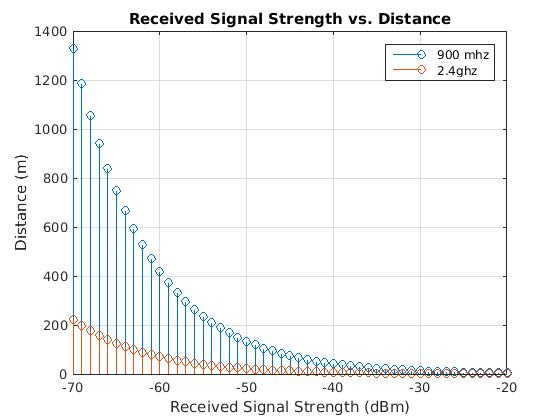
\includegraphics[width=\linewidth]{figures/rss-vs-distance.jpg}
       \caption{\label{fig:log-distance}RSSI readings of NLoS and LoS APs acquired with a stationary agent}
    \end{figure}

    However, in order to obtain $\hat{d}$, the path loss exponent $n$ should be estimated from the collected data.
    Let $\mathbf{m} = \{m_i | i=1 \ldots n_{location} \}$ and $\mathbf{X} = \{ \mathbf{x}_i | i = 1 \ldots n_{location}\}$ be the fingerprints collected during surveying and corresponding locations, respectively.
    The approximated propagation function for each anchor nodes can be written as $f_{\hat{d}}(\mathbf{x}, m_i, n): \mathbf{M} \mapsto \mathbf{X}$.

    \begin{equation}
      n^* = \argmin_n \{\norm{\mathbf{X}}_2 - f_{\hat{d}}(\mathbf{X}, \mathbf{m}, n)\}
    \end{equation}


    % Indoor localization is an important problem in which an object of interest, i.e.\ a robot in our framework, suited with different sensors localizes itself in an indoor environment where there is no global positioning information is available.
    % \textit{The complexity of the problem significantly \# \textit{exponentially} increases as NLoS of reference AP's, presence of hard-constraints, in particular infrasractural elements such as walls and doors, noisy nature of the signals, and dynamic environments.}~\cite{liu2007survey}
    % \textit{As robotic systems find more applications in indoor areas where dynamic objects, such as other robots and humans, often coexist, it increasingly becomes important to safely and accurately localize the agent.} %where there is no reliable global positioning system is available.}
    % % \textit{Maybe co-robots can be mentioned.}
    % Thus, a great amount of interest has been showed from both academia and industry.
    % \# \textit{Do I really emphasize industry academia, actually this is a good opportunity to mention iBeacon from Apple}
    % The indoor localization systems based WiFi signal can be mainly categorized undepngr two categories: fingerprinting and model-based methods~\cite{hossain2015survey}.
    % We'll, however, only cover the fingerprinting technique due to the increasing popularity of the technique.



    % \begin{itemize}
    %   \item CSI-related special \\
    %     hardware requirement
    %   \item Propagation-modelling \\
    %     multi-path effect difficult to model
    %   \item Fingerprinting \\
    %     An emerging area learning fingerprints is deep learning~\cite{gao2015channel}
    % \end{itemize}
